\documentclass[aspectratio=169]{beamer}
\usetheme{Bruno}
\setbeamertemplate{footline}[frame number]
\usepackage{comment}
\usepackage{graphicx}
\usepackage{booktabs}
\usepackage{tabularx}
\graphicspath{{images/}{../se/OA/}{../se/SA/}{../se/LA/}{../se/PA/}}

\title[2026-04-23 CDR]{ASADA Paso Ancho 2026-04-23 CDR}
\author[Lab Delta]{Laboratorio Delta}
\date{2026-04-23}

\begin{document}

% ═══════════════════════════════════════════════════════════════════════
% TITLE
% ═══════════════════════════════════════════════════════════════════════
\begin{frame}
    \begin{center}
        {\LARGE \textbf{\inserttitle}} \\
        \vspace{0.5cm}
        {\insertauthor} \\
        \vspace{0.25cm}
        
\includegraphics[height=2.3cm]{logo_delta.png} \raisebox{0.4cm}{
\includegraphics[height=1.3cm]{logo_tec.jpg}} \\
    \end{center}
\end{frame}

% ═══════════════════════════════════════════════════════════════════════
% CRITICAL DESIGN REVIEW
% ═══════════════════════════════════════════════════════════════════════
\begin{frame}
    \begin{center}
        {\LARGE \textbf{Critical Design Review}} \\
        \vspace{0.5cm}
        {ASADA Paso Ancho} \\
        \vspace{0.25cm}
    \end{center}
\end{frame}

\begin{frame}
    \frametitle{Critical Design Review}

    {\textbf{Contents}}
    \begin{itemize}
        \item Physical Architecture
    \end{itemize}
    \vspace{0.25cm}
    {\textbf{Goals}}
    \begin{itemize}
        \item Approve Physical Architecture
    \end{itemize}
\end{frame}

\begin{frame}
    \frametitle{Potable Water Regulation No. 38924-S}

    \begin{columns}[T]
        \begin{column}{0.3\textwidth}
            \textbf{Artículo 11.} Todo ente operador de un sistema de suministro de agua, está obligado a confeccionar reportes de la calidad del agua potable y presentarlos \textbf{semestralmente}...
        \end{column}
        \begin{column}{0.7\textwidth}
            \centering
            \begin{figure}
                \centering
                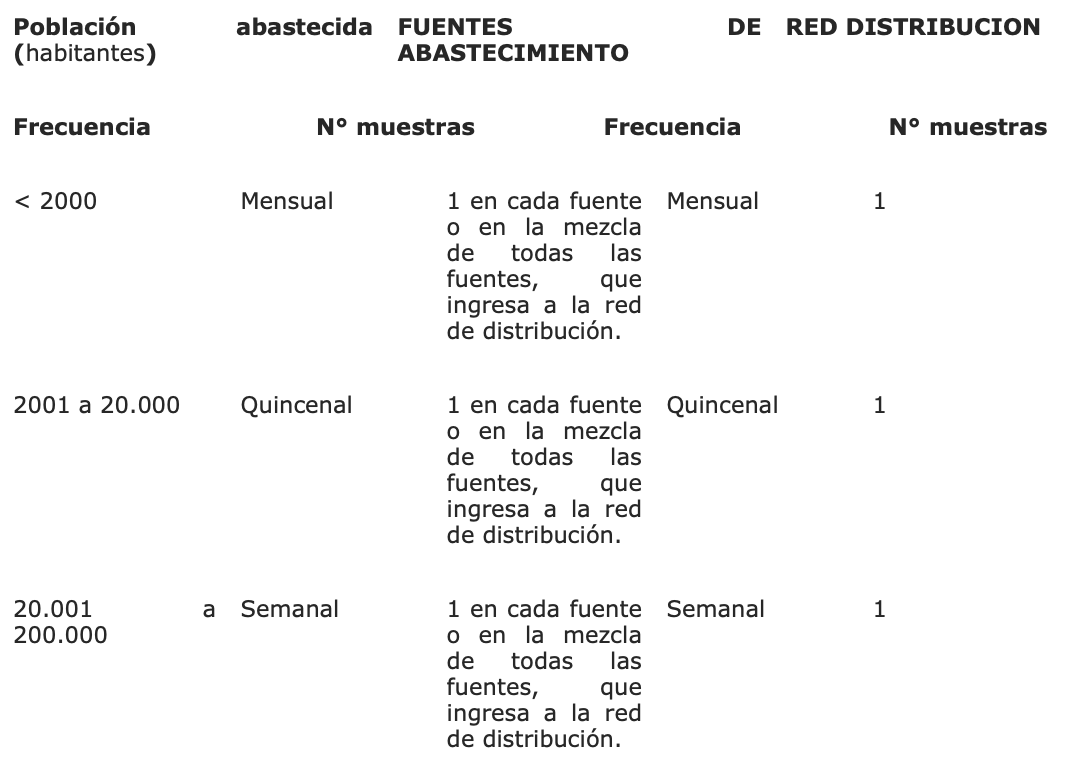
\includegraphics[width=0.7\textwidth]{Cuadro_B.1.png}
                \caption{CUADRO B.1 Frecuencia mínima de muestreo y número de muestras a recolectar en las FUENTES DE ABASTECIMIENTO Y RED DE DISTRIBUCION para el CONTROL OPERATIVO (CO)}
            \end{figure}
        \end{column}
    \end{columns}
\end{frame}

\begin{frame}
    \frametitle{\small Physical Architecture: Power Infrastructure}

    \begin{figure}
        \centering
        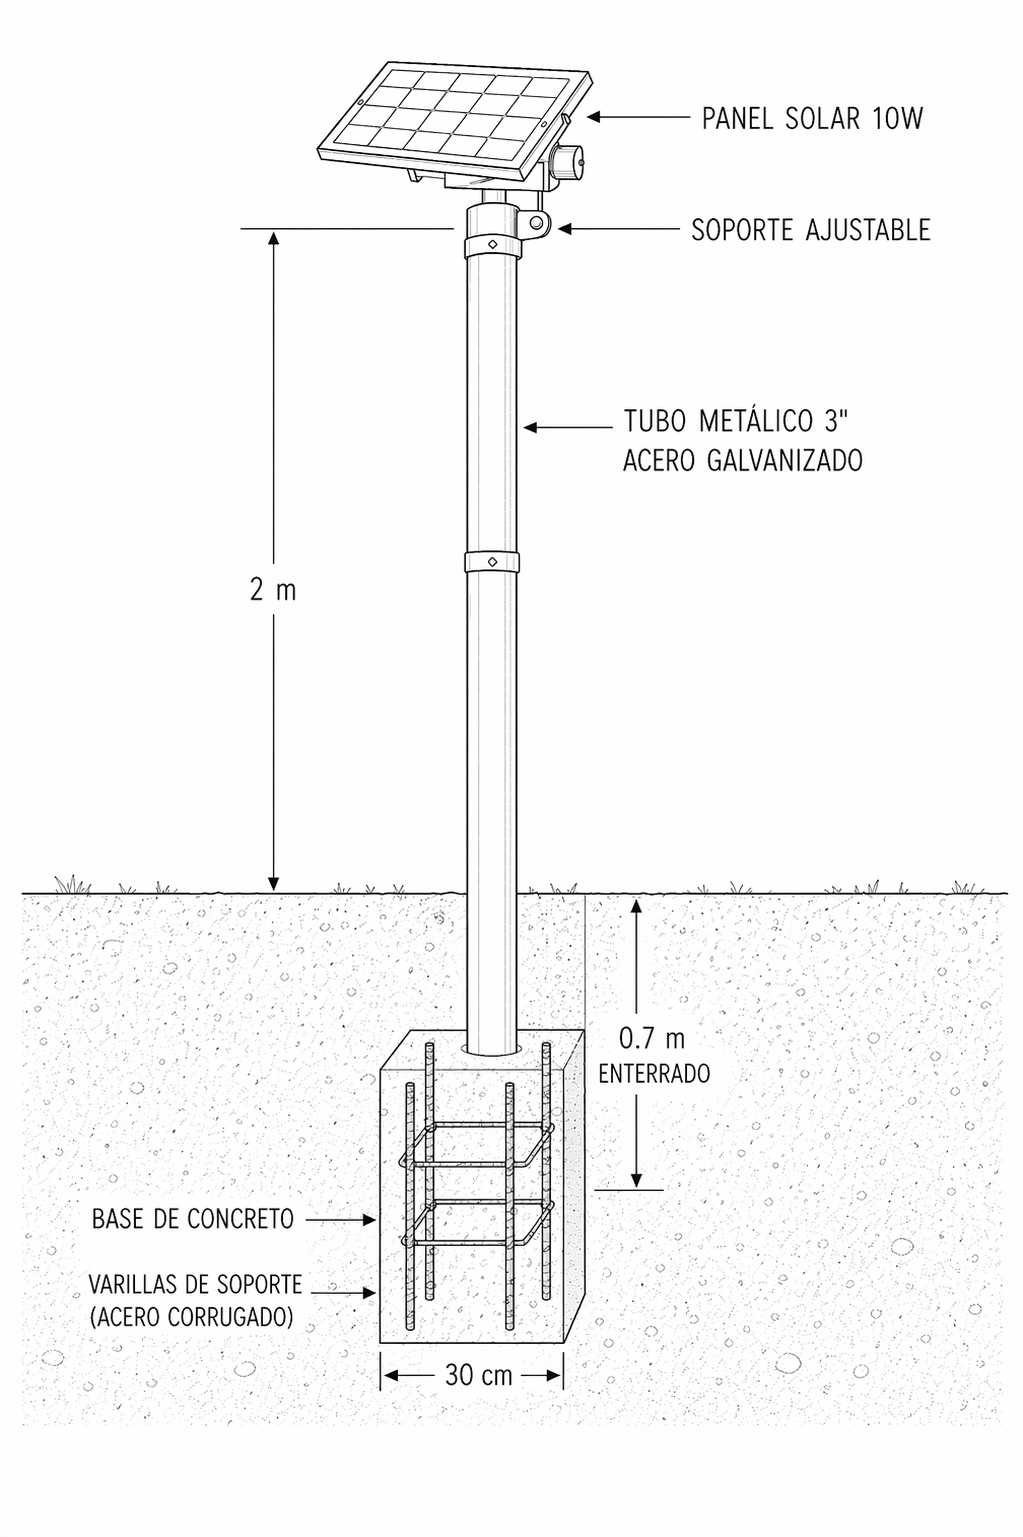
\includegraphics[width=\textwidth,height=0.74\textheight,keepaspectratio]{Puesta_en_marcha.png}
    \end{figure}
\end{frame}

\begin{frame}
    \frametitle{\small Physical Architecture: Physical Security}
    \framesubtitle{On-site piping enclosure has a lock}

    \begin{figure}
        \centering
        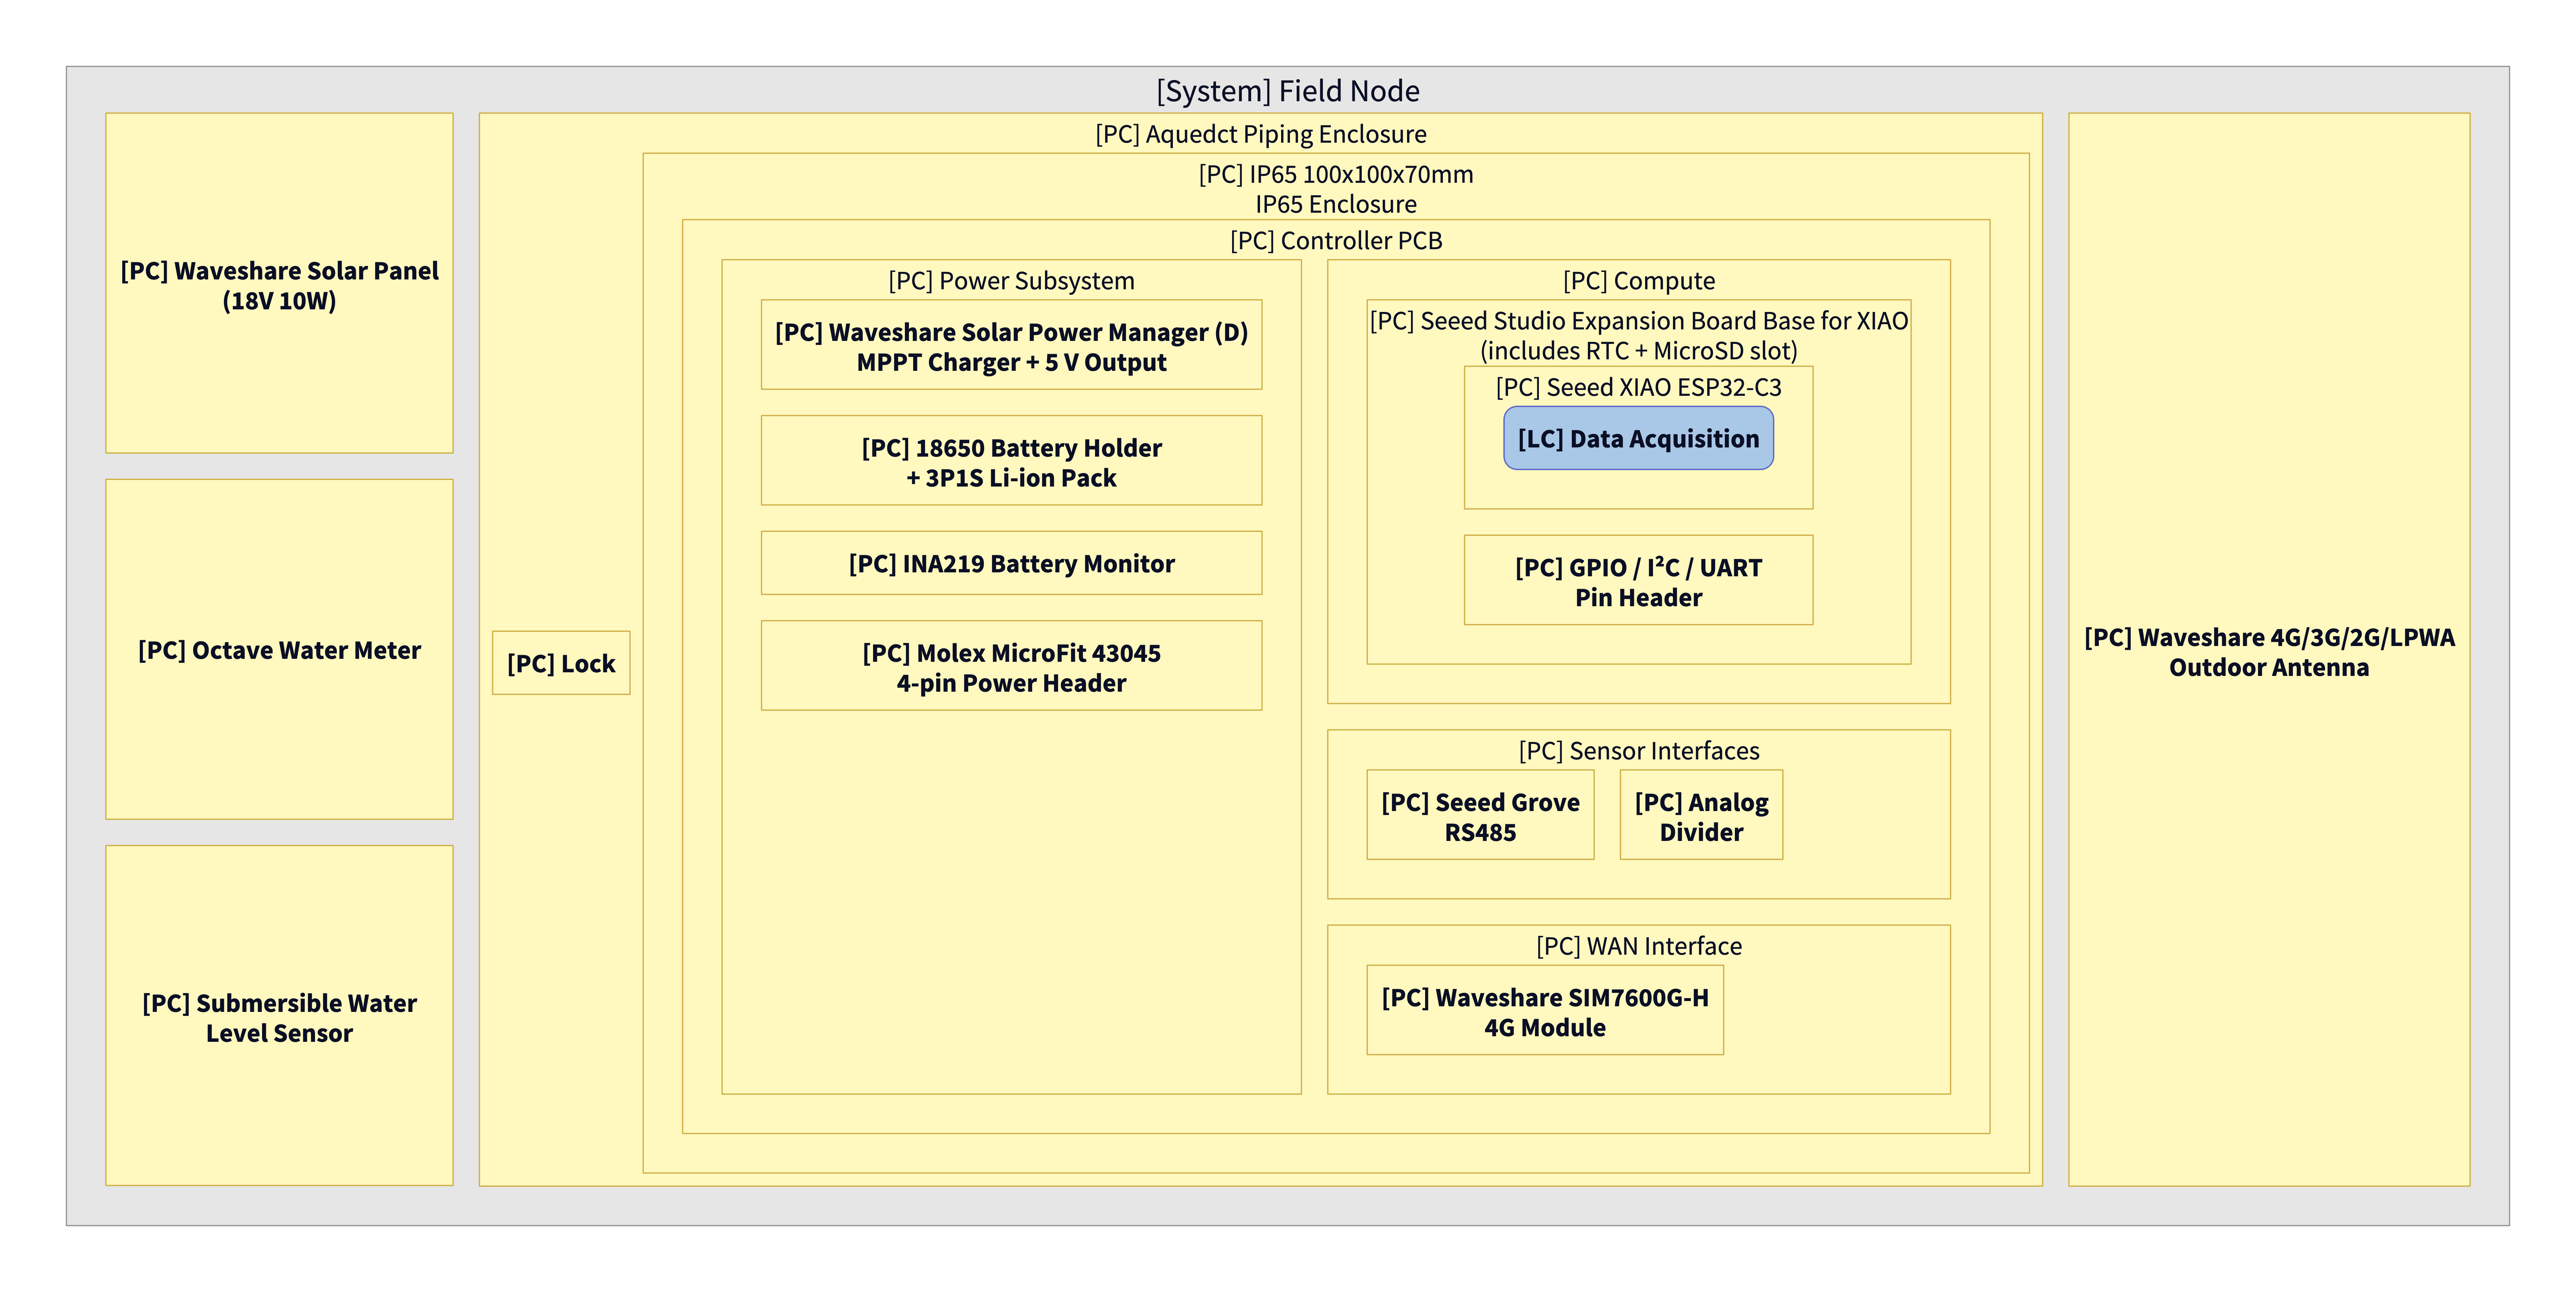
\includegraphics[width=\textwidth,height=0.74\textheight,keepaspectratio]{Field Node PA without PLs.d2.png}
    \end{figure}
\end{frame}

\begin{frame}
    \frametitle{\small Physical Architecture: Firewall, SIEM, Tamper Detection}

    \begin{figure}
        \centering
        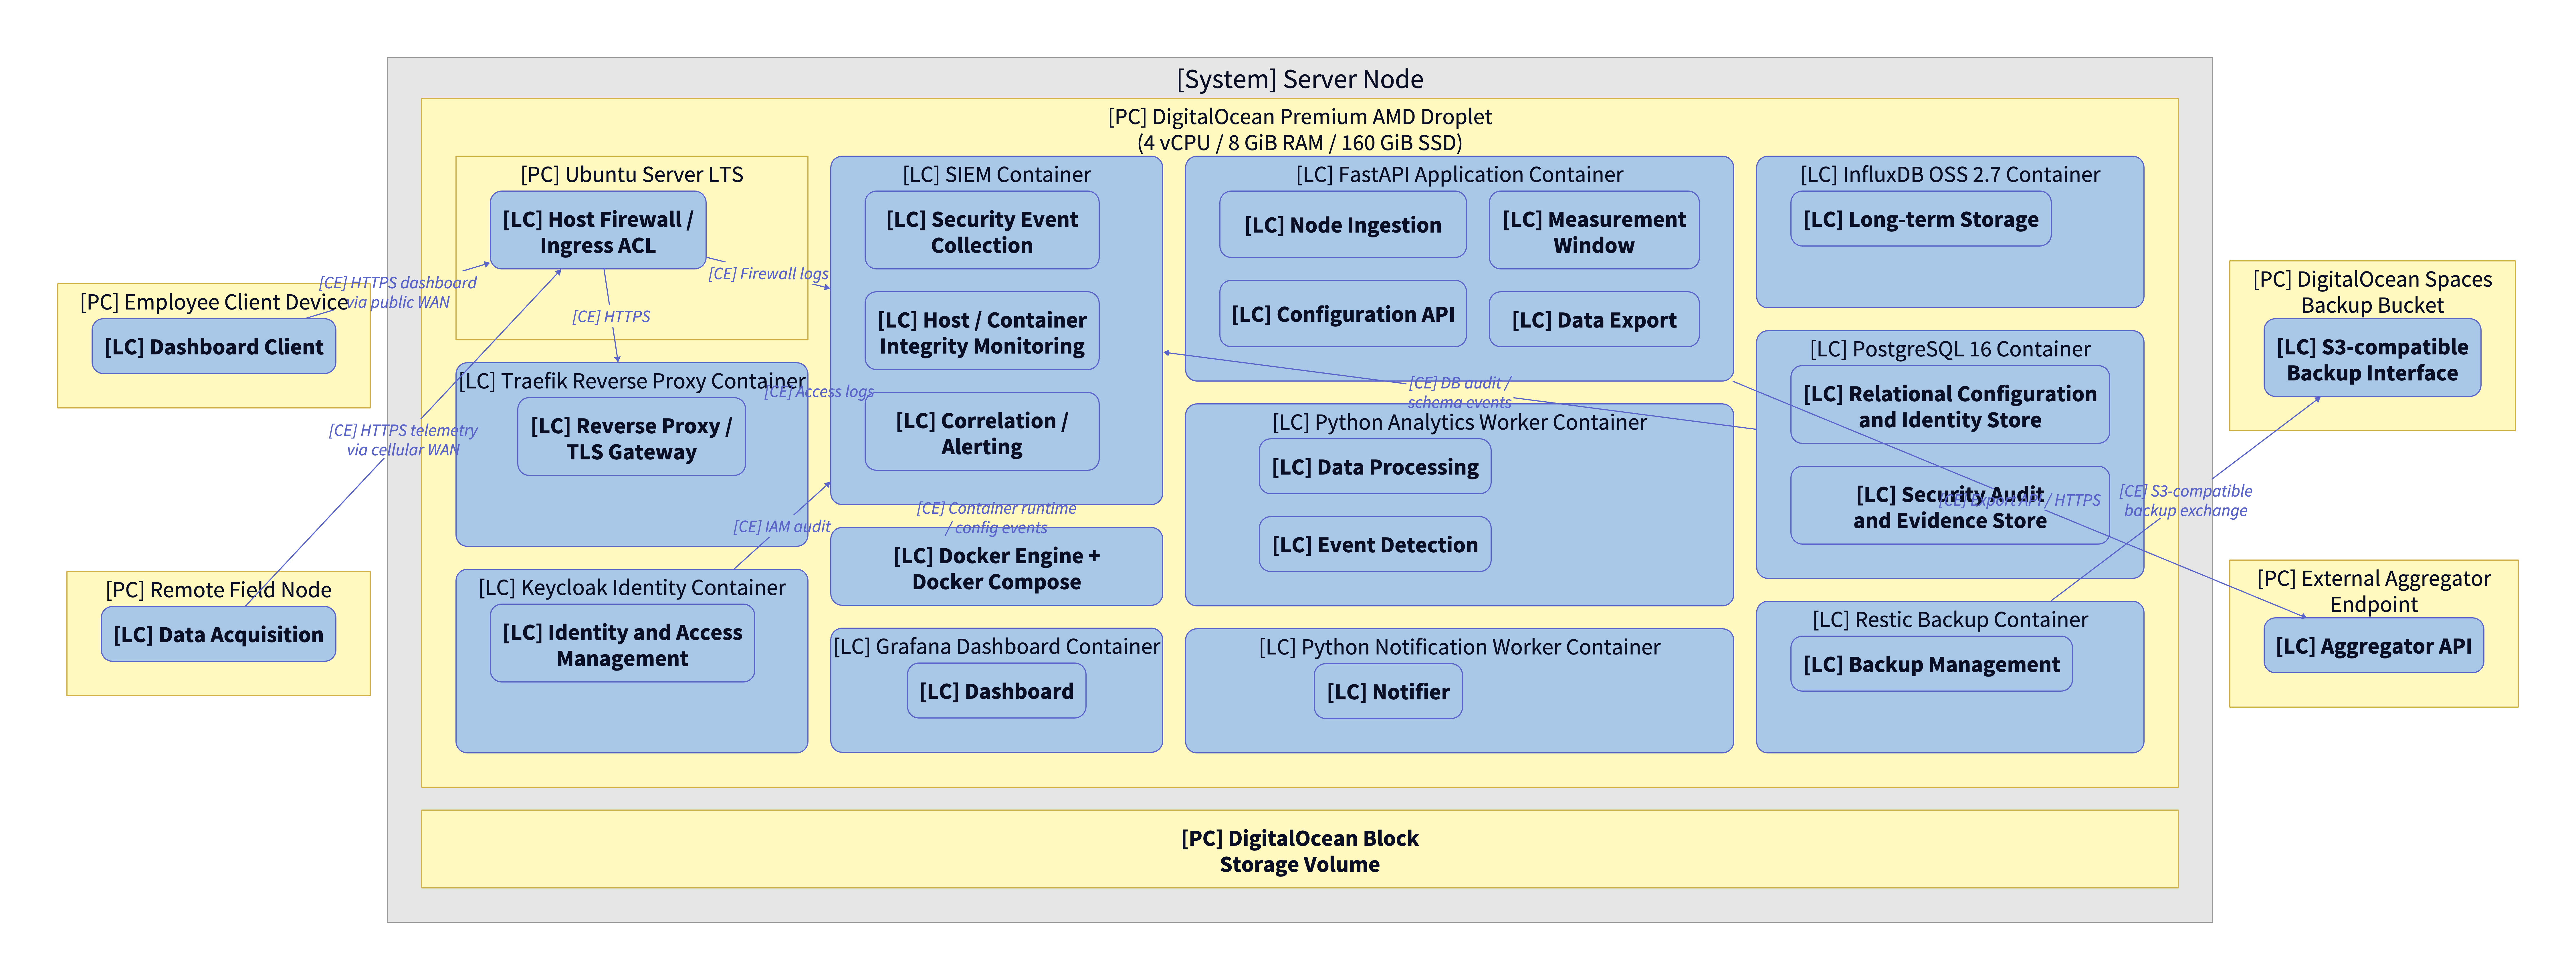
\includegraphics[width=\textwidth,height=0.74\textheight,keepaspectratio]{Server Node PA.d2.png}
    \end{figure}
\end{frame}

\begin{frame}
    \frametitle{\small Feared Event Scenario: Server Tamper Detection}
    \framesubtitle{Host, container, and audit deviations become alerts and reviewable evidence}

    \begin{figure}
        \centering
        
\includegraphics[width=\textwidth,height=0.72\textheight,keepaspectratio]{scenario_detect_server_tamper.d2.png}
    \end{figure}
\end{frame}

\begin{frame}
    \frametitle{Bill of Materials (Field Node)}

    \footnotesize
    \begin{tabularx}{\textwidth}{l X}
        \toprule
        Component & Part \\
        \midrule
        Microcontroller    & Seeed XIAO ESP32-C3 \\
        Expansion board    & Seeed Studio Expansion Base for XIAO (RTC + MicroSD) \\
        RS-485 interface   & Seeed Grove RS485 \\
        LTE modem          & Waveshare SIM7600G-H 4G Module \\
        Cellular antenna   & Waveshare 4G/3G/2G/LPWA Outdoor Antenna \\
        Solar panel        & Waveshare Solar Panel 18\,V 10\,W \\
        Power manager      & Waveshare Solar Power Manager (D) --- MPPT + 5\,V output \\
        Battery            & 18650 3P1S Li-ion Pack + Holder \\
        Battery monitor    & INA219 \\
        Level sensor       & Submersible Water Level Sensor (0.5--4.5\,V) \\
        Flow meter         & Octave Water Meter (existing, RS-485 Modbus) \\
        \bottomrule
    \end{tabularx}
\end{frame}

\begin{frame}
    \frametitle{Power Subsystem Components}

    \begin{columns}[T]
        \begin{column}{0.25\textwidth}
            \centering
            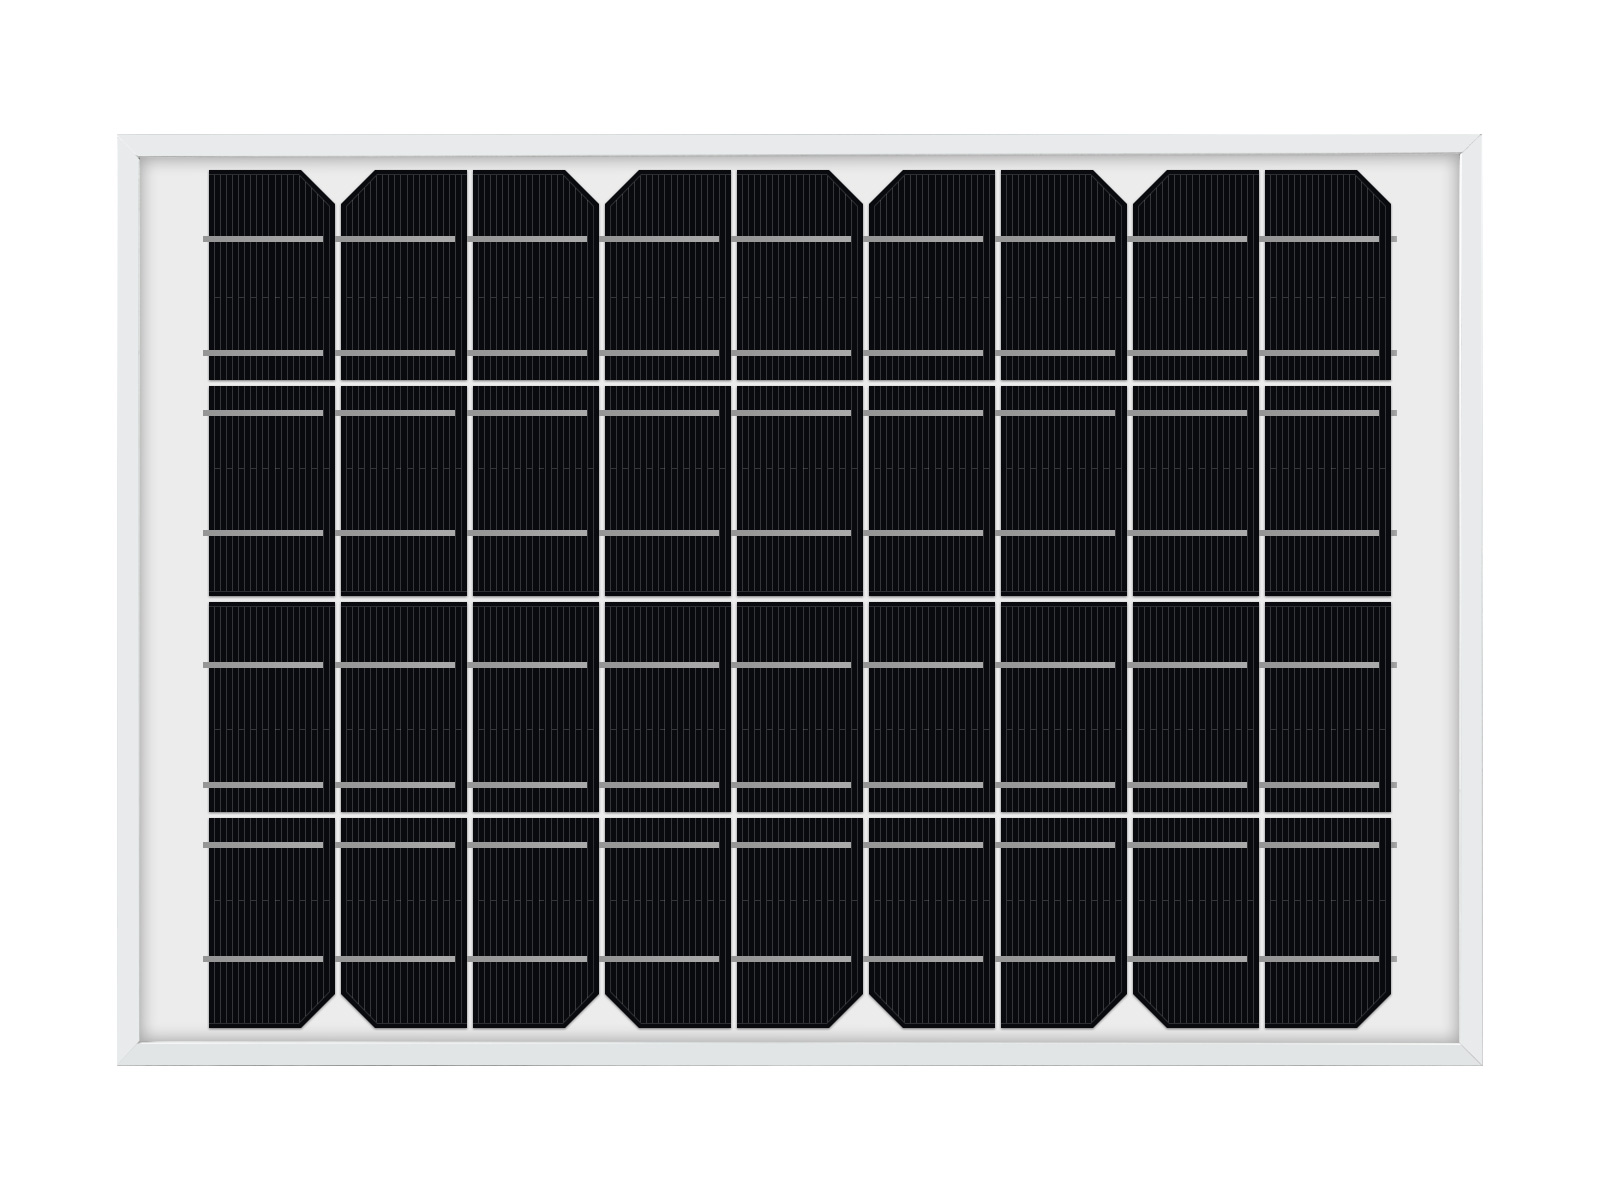
\includegraphics[width=\linewidth,height=2.8cm,keepaspectratio]{prod_solar_panel.jpg} \\[0.2em]
            {\small \textbf{Solar Panel 18\,V 10\,W}} \\
            {\footnotesize Waveshare} \\[0.2em]
            {\large \$11.99}
        \end{column}
        \begin{column}{0.25\textwidth}
            \centering
            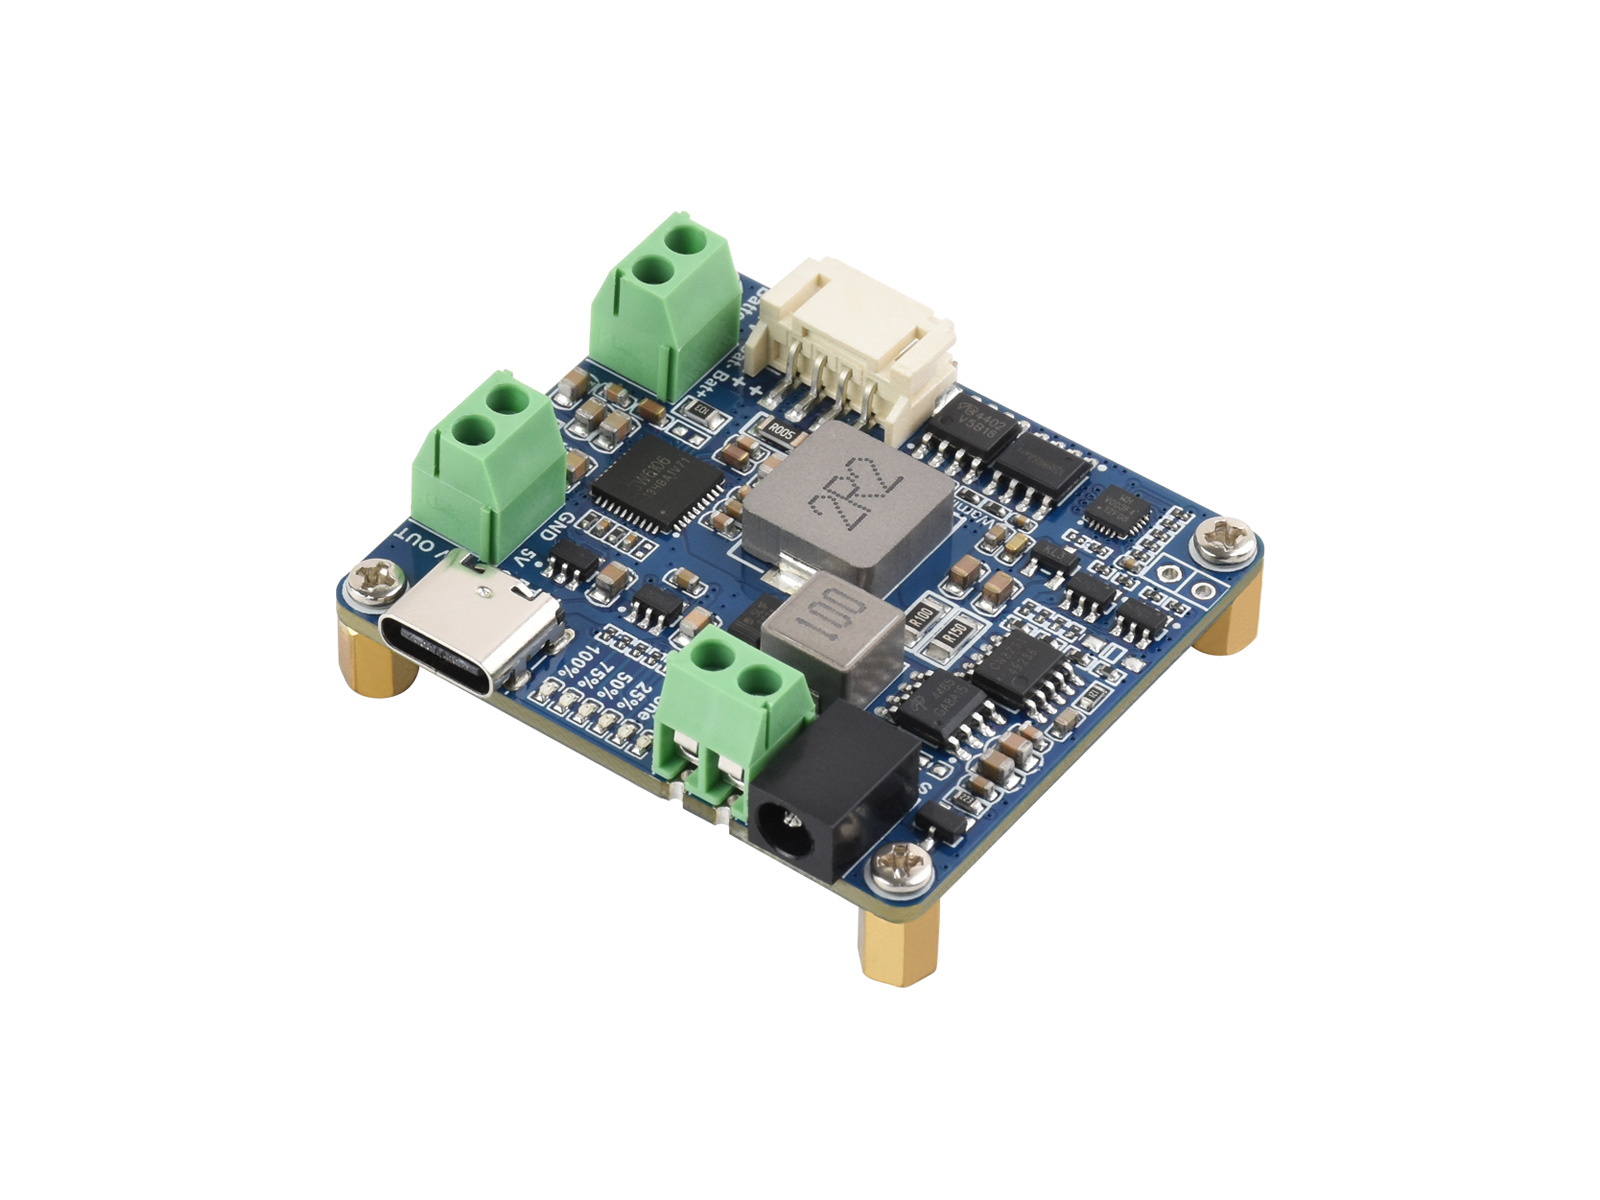
\includegraphics[width=\linewidth,height=2.8cm,keepaspectratio]{prod_solar_manager.jpg} \\[0.2em]
            {\small \textbf{Solar Power Manager (D)}} \\
            {\footnotesize Waveshare} \\[0.2em]
            {\large \$12.99}
        \end{column}
        \begin{column}{0.25\textwidth}
            \centering
            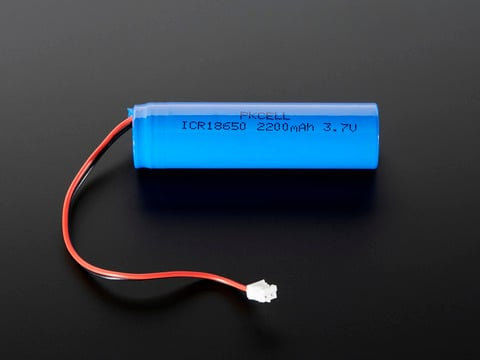
\includegraphics[width=\linewidth,height=2.8cm,keepaspectratio]{prod_18650.jpg} \\[0.2em]
            {\small \textbf{18650 Li-ion Cell $\times$3}} \\
            {\footnotesize 3.7\,V 2200\,mAh, 3P1S pack} \\[0.2em]
            {\large \$9.95 $\times$ 3}
        \end{column}
        \begin{column}{0.25\textwidth}
            \centering
            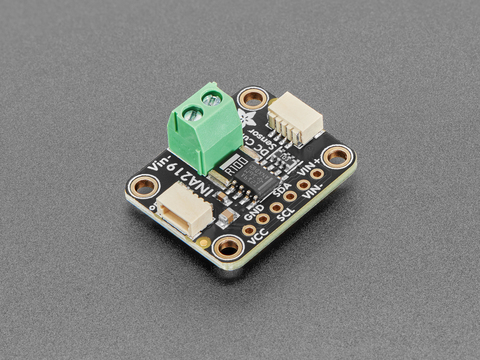
\includegraphics[width=\linewidth,height=2.8cm,keepaspectratio]{prod_ina219.jpg} \\[0.2em]
            {\small \textbf{INA219 Battery Monitor}} \\
            {\footnotesize Adafruit breakout} \\[0.2em]
            {\large \$9.95}
        \end{column}
    \end{columns}

    \vfill
    \centering
    \footnotesize
    Subtotal (power subsystem): \textbf{\$64.78} \quad|\quad
    Sources: Waveshare, Adafruit
\end{frame}

\begin{frame}
    \frametitle{Server Runtime Services}

    \begin{columns}[T,onlytextwidth]
        \begin{column}{0.32\textwidth}
            \centering
            
\includegraphics[height=0.55cm]{server_services/traefikproxy.png} \\[0.05em]
            {\footnotesize \textbf{Traefik}} \\[0.1em]
            {\tiny
            • Edge TLS termination \\
            • Single controlled ingress path
            }

            \vspace{0.2em}
            
\includegraphics[height=0.55cm]{server_services/keycloak.png} \\[0.05em]
            {\footnotesize \textbf{Keycloak}} \\[0.1em]
            {\tiny
            • OIDC SSO and token issuance \\
            • Password handling isolated from app containers
            }
        \end{column}
        \begin{column}{0.32\textwidth}
            \centering
            
\includegraphics[height=0.55cm]{server_services/grafana.png} \\[0.05em]
            {\footnotesize \textbf{Grafana}} \\[0.1em]
            {\tiny
            • Keycloak-backed SSO \\
            • RBAC can restrict threshold editing
            }

            \vspace{0.2em}
            
\includegraphics[height=0.55cm]{server_services/fastapi.png} \\[0.05em]
            {\footnotesize \textbf{FastAPI}} \\[0.1em]
            {\tiny
            • Auditable ingestion/config/export API \\
            • Token, node-identity, and input validation
            }
        \end{column}
        \begin{column}{0.32\textwidth}
            \centering
            
\includegraphics[height=0.55cm]{server_services/influxdb.png} \\[0.05em]
            {\footnotesize \textbf{InfluxDB OSS 2.7}} \\[0.1em]
            {\tiny
            • Bucket and token separation \\
            • Write-only node tokens; read-only export tokens
            }

            \vspace{0.2em}
            
\includegraphics[height=0.55cm]{server_services/postgresql.png} \\[0.05em]
            {\footnotesize \textbf{PostgreSQL 16}} \\[0.1em]
            {\tiny
            • Central config and identity store \\
            • Kept off the public internet
            }
        \end{column}
    \end{columns}

    \vfill
    \centering
    {\tiny Additional custom containers: Python analytics worker, notification worker, and Restic backup job.}
\end{frame}

\begin{frame}
    \frametitle{Main Reliability Scenarios}

    \begin{columns}[T,onlytextwidth]
        \begin{column}{0.49\textwidth}
            \centering
            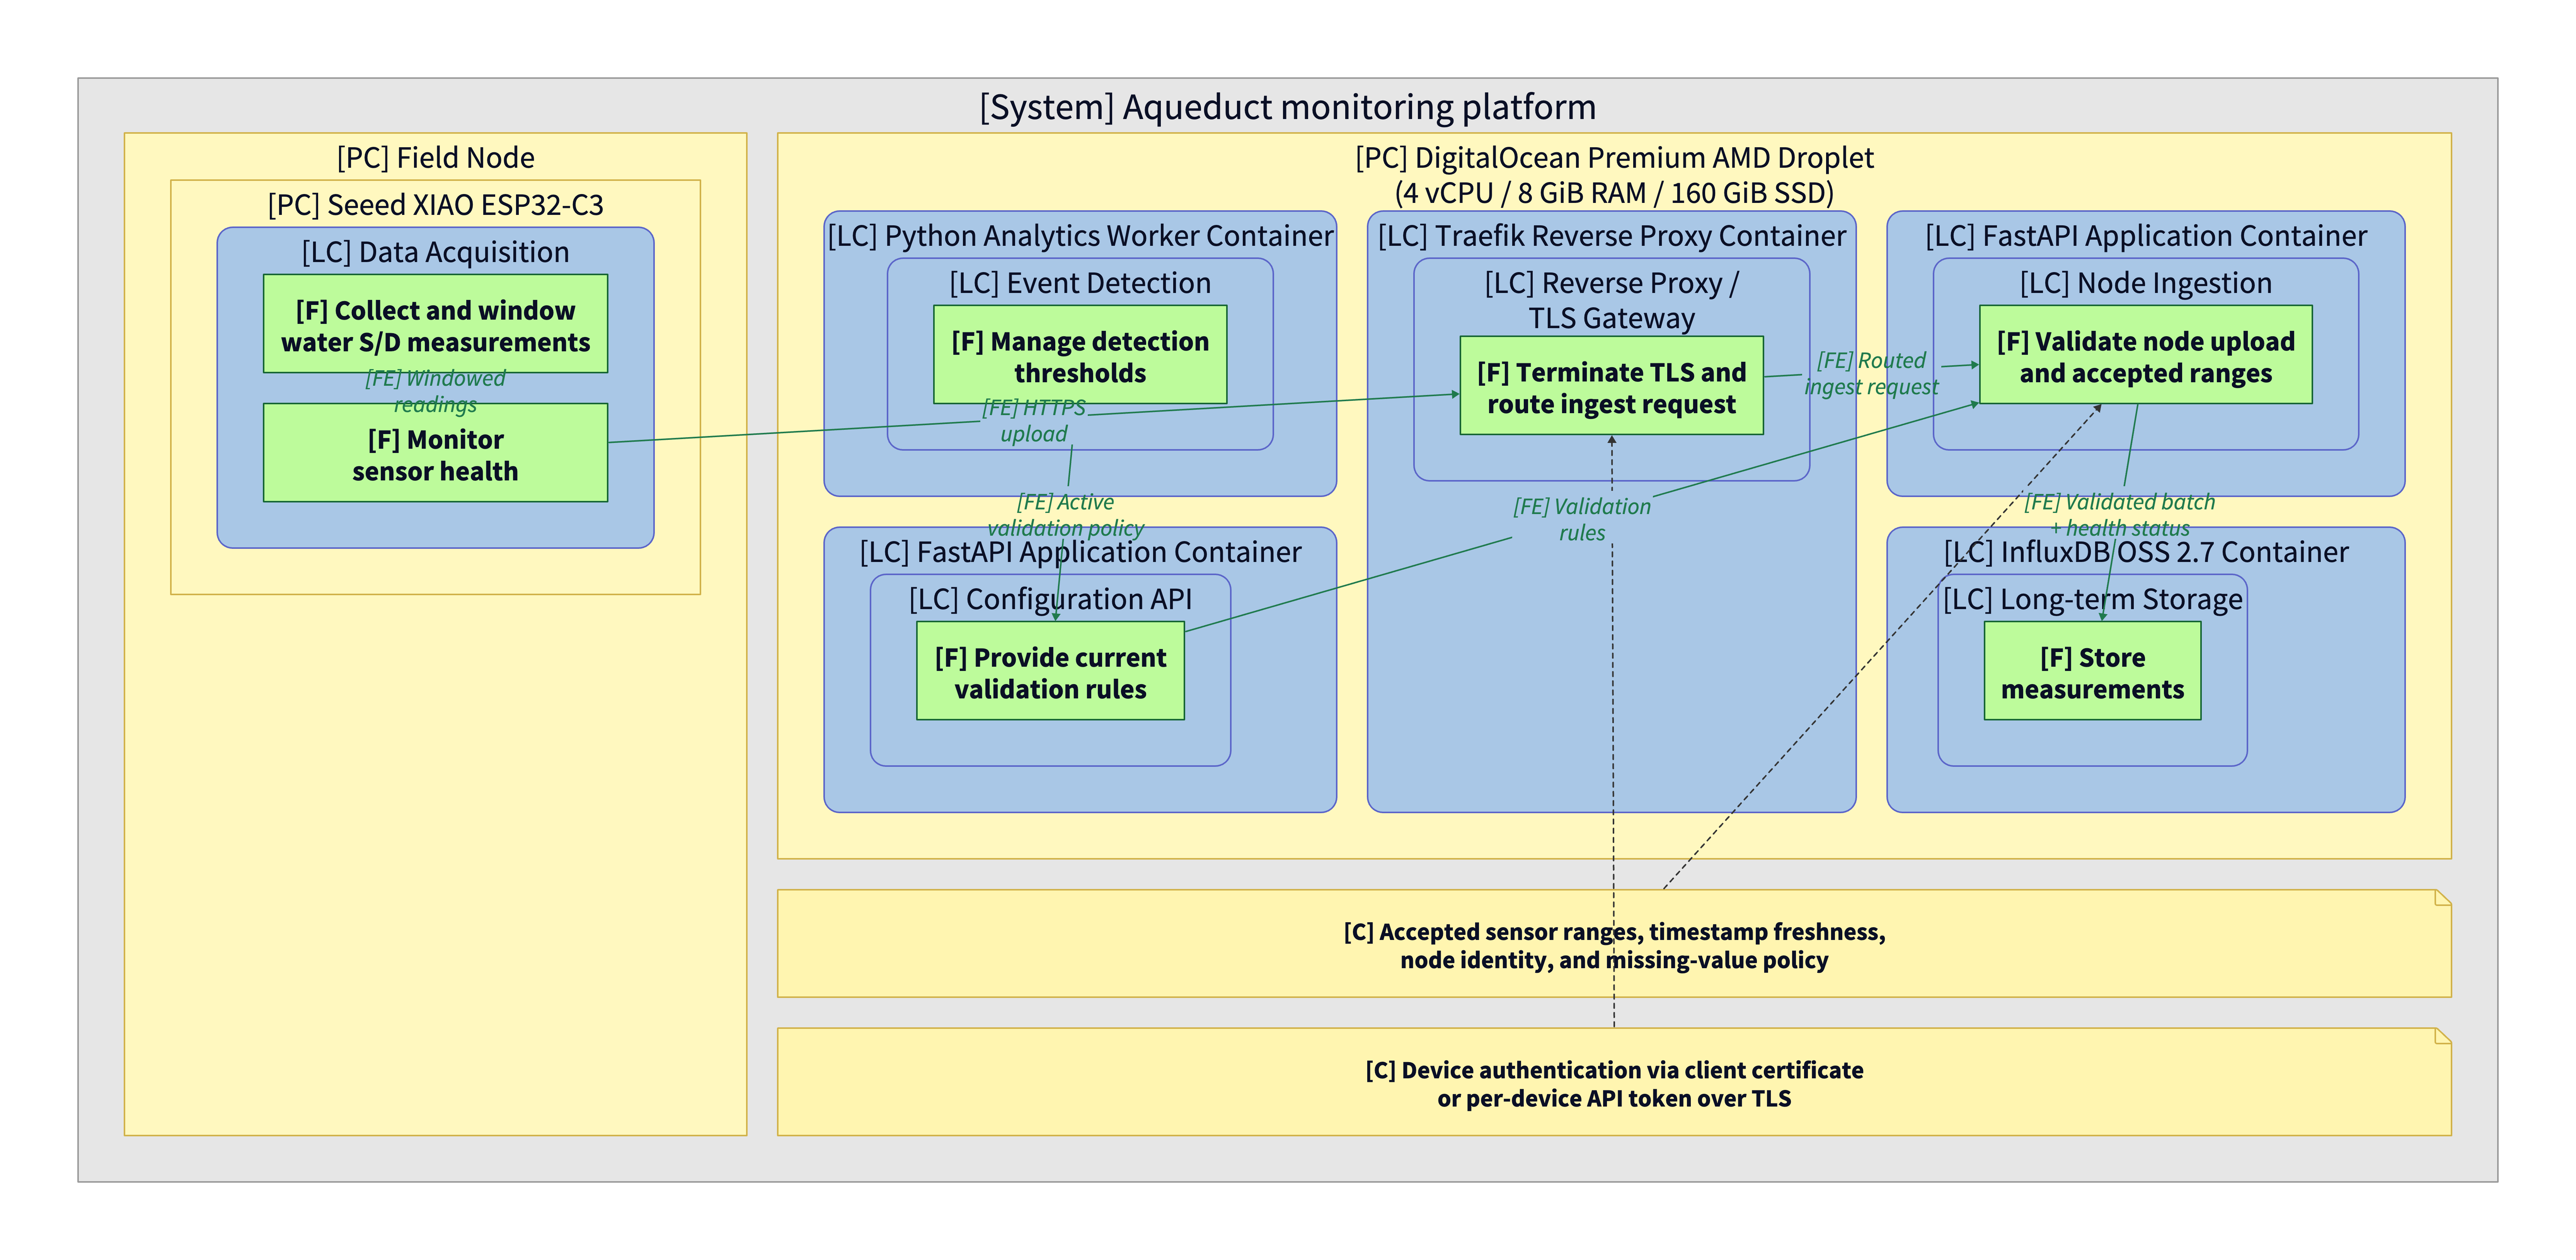
\includegraphics[width=\linewidth,height=0.40\textheight,keepaspectratio]{scenario_ingest_validate_node_data.d2.png} \\
            {\small \textbf{Upload path}} \\
            {\scriptsize nominal upload + reject stale / malformed / unauthorized data}
        \end{column}
        \begin{column}{0.49\textwidth}
            \centering
            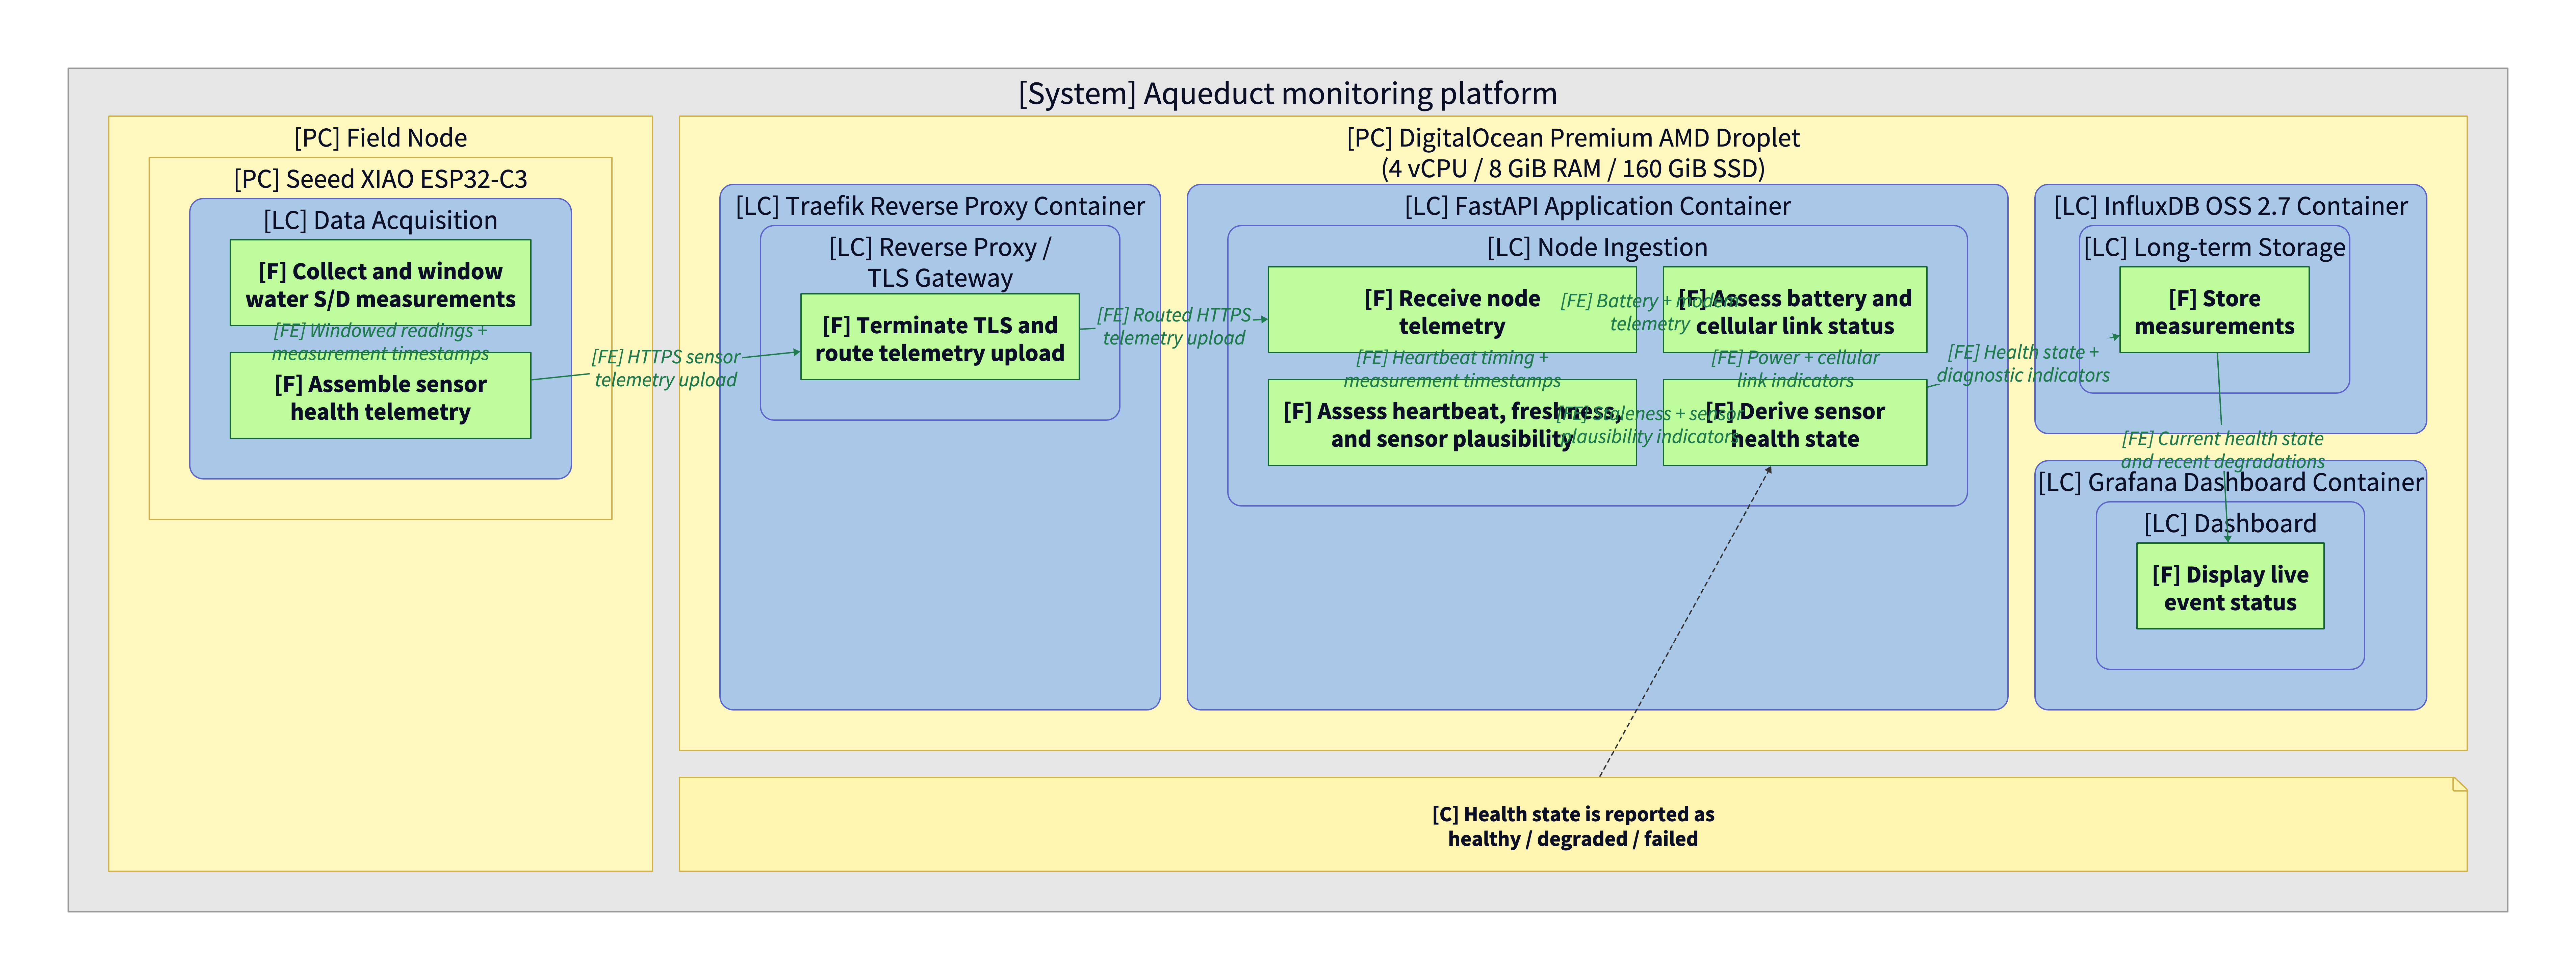
\includegraphics[width=\linewidth,height=0.40\textheight,keepaspectratio]{scenario_monitor_sensor_health.d2.png} \\
            {\small \textbf{Health path}} \\
            {\scriptsize sensor plausibility + battery + LTE + degraded / failed state}
        \end{column}
    \end{columns}

    \vspace{0.15cm}
    \begin{columns}[T,onlytextwidth]
        \begin{column}{0.38\textwidth}
            \centering
            \includegraphics[width=\linewidth,height=0.18\textheight,keepaspectratio]{FV2_bench_field_node.d2.png}
        \end{column}
    \end{columns}
\end{frame}


\end{document}
